\chapter{PREESM}
\label{chapter:preesm}
In this chapter the PREESM rapid prototyping framework is introduced. First an
overview of the framework is given. Next the internal program representation in
PREESM is introduced.

\section{PREESM Overview}
\label{sec:preesmover}
The PREESM rapid prototyping framework for multicore development was used to
create a workload application for the thesis experiment described in
\ref{sec:firstexperiment}. Dataflow Models of Computation (MoC), discussed in
section \ref{sec:dataflow}, are used in PREESM to build a representation of the
application. The application is divided into parallel actors, which communicate
through First In, First Out (FIFO) data queues. The actors are manually created
by the application designer in the target language. PREESM provides graphical
tools for editing the dataflow diagram and it generates a static schedule for
multicore platforms that is guaranteed to be deadlock free. PREESM combines the
generated and manually created code into a multicore executable
\cite{pelcat2014preesm}. The code generation can be configured through graphical
tools that provide hints to the schedule generation about the execution time of
different actors and rules on which cores they can be executed. A PREESM
dataflow diagram is presented in figure \ref{preesm_example}.

\begin{figure}[h!] \label{preesm_example} \begin{center}
    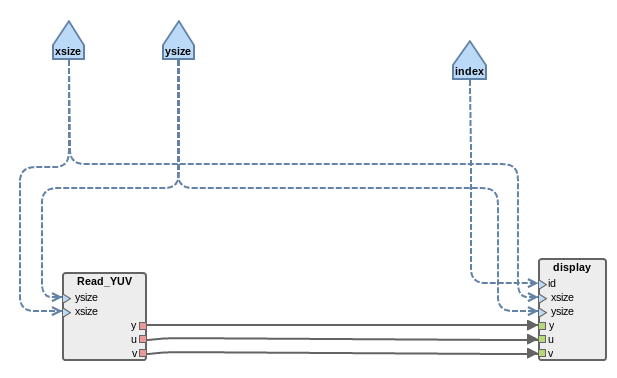
\includegraphics[width=0.99\textwidth]{images/example_preesm_diagram.png}
    \caption{A simple dataflow diagram used by PREESM} \end{center}
\end{figure}

In the experiment \ref{sec:firstexperiment} a baseline application for comparison
with OpenEM was needed. PREESM was selected because it is capable of code
generation for TMS320C6678, introduced in chapter \ref{chapter:c6678}, and its
simple and fast workflow.

\section{PREESM Internal Representations}
\label{sec:dataflow}
PREESM applications are created by combining inputs of two different
internal representations and manually created source code. The two internal
representations are described here: first the PREESM algorithm representation
PiSDF and second the PREESM hardware model.

\subsection{PREESM Algorithm Representation}
The PREESM applications are defined using the Parameterized and Interfaced
Synchronous Dataflow Model of Computation (PiSDF)\cite{pelcat2014preesm}.

Dataflow Model of Computation (MoC) is a directed graph where each node
represents a function and the arcs are the only possible paths the data can
traverse in the graph. In the generic Dataflow MoC the number of tokens produced
or consumed by an actor is not known before execution. For example an actor may
have two output paths and it may choose to produce an output token conditionally
to either one (or both) of the paths. In contrast in Synchronous Data Flow
(SDF) MoC each actor produces and consumes a pre-determined number of tokens.
\cite{lee1987synchronous} A more thorough explanation of Dataflow MoCs can be
found in \cite{lee2015introduction}.

PREESM uses an extended version of SDF called PiSDF \cite{pelcat2014preesm}.
PiSDF extends SDF by providing hierarchical graphs based on interfaces and by
introducing parameterized actors. An actor in PiSDF can be replaced by a
subgraph, which has input and output interfaces. The interfaces insulate the
hierarchy levels in terms of schedulability analysis. The parameters are used
to reconfigure the production and consumption rates of the actors.
\cite{desnos2013pimm} An example of a PiSDF graph is presented in figure
\ref{preesm_example}. The parameters of the PiSDF model are presented at the
top of the figure as pentagons connected to the actors with dashed lines. The
actors have input and output ports for parameters and data. The ports define
the input and output interfaces of the actors. The actual data paths are the
arcs connecting the actors in the bottom of the figure.

\subsection{PREESM Platform Representation}
The PREESM code generation is aware of the target hardware platform. PREESM
uses System-Level Architecture Model (S-LAM) \cite{pelcat2009system} to
describe the target architecture. S-LAM is designed specifically to provide
architecture models of high asbtraction level for rapid prototyping purposes.
S-LAM is suitable for modeling heterogeneous architectures as a S-LAM can
contain different types of computational resources and communication links. In
PREESM the speeds of the connections in the S-LAM are calculated and taken into
account when creating a static schedule. \cite{pelcat2009system}

PREESM provides graphical tools for editing the S-LAM. For example the S-LAM
representing the TMS320C6678 used in experiment \ref{sec:firstexperiment} is
quite simple consisting of eight c6678 cores connected through shared memory.

\section{PREESM Scheduling}
\label{sec:preesmsched}
A general problem in the design of multicore applications is efficient
scheduling. The PREESM framework generates a schedule for multicore platforms
using the \textit{List} and \textit{Fast} scheduling methods explained in
\cite{kwok1997high}. The PREESM framework focuses on latency dominated systems
where respecting the latency constraints guarantees fulfilment of the throughput
constraint \cite{pelcat2014preesm, ghamarian2006throughput}. Because the
scheduler only considers the latency of the execution, the iterations of the
algorithm are not interleaved. Instead, all cores are synchronized between the
iterations with a barrier. Intra-iteration interleaving is supported by the
PREESM scheduler. \cite{pelcat2014preesm} An example of the intra-iteration
interleaving is given in the software pipelining tutorial available at
\cite{preesm}. The estimated execution times for each actor are provided by the
user. PREESM framework visualizes the generated schedule with a gantt chart. An
example gantt chart is presented in figure \ref{preesm_gantt}.
